subsection{Concept of execution}

This paragraph describes the concept of execution among the system components, which are shown in Figure.~{fig:Component_overview}. Since the relations between system 
components do not change dynamically, this section will describe the execution of a central scenario: Threat detected.

\paragraph{Threat detected scenario}\mbox{}\\
This scenario unfolds when the sensors detect a missile threat.



%\begin{figure}[h]
%	\centering
%	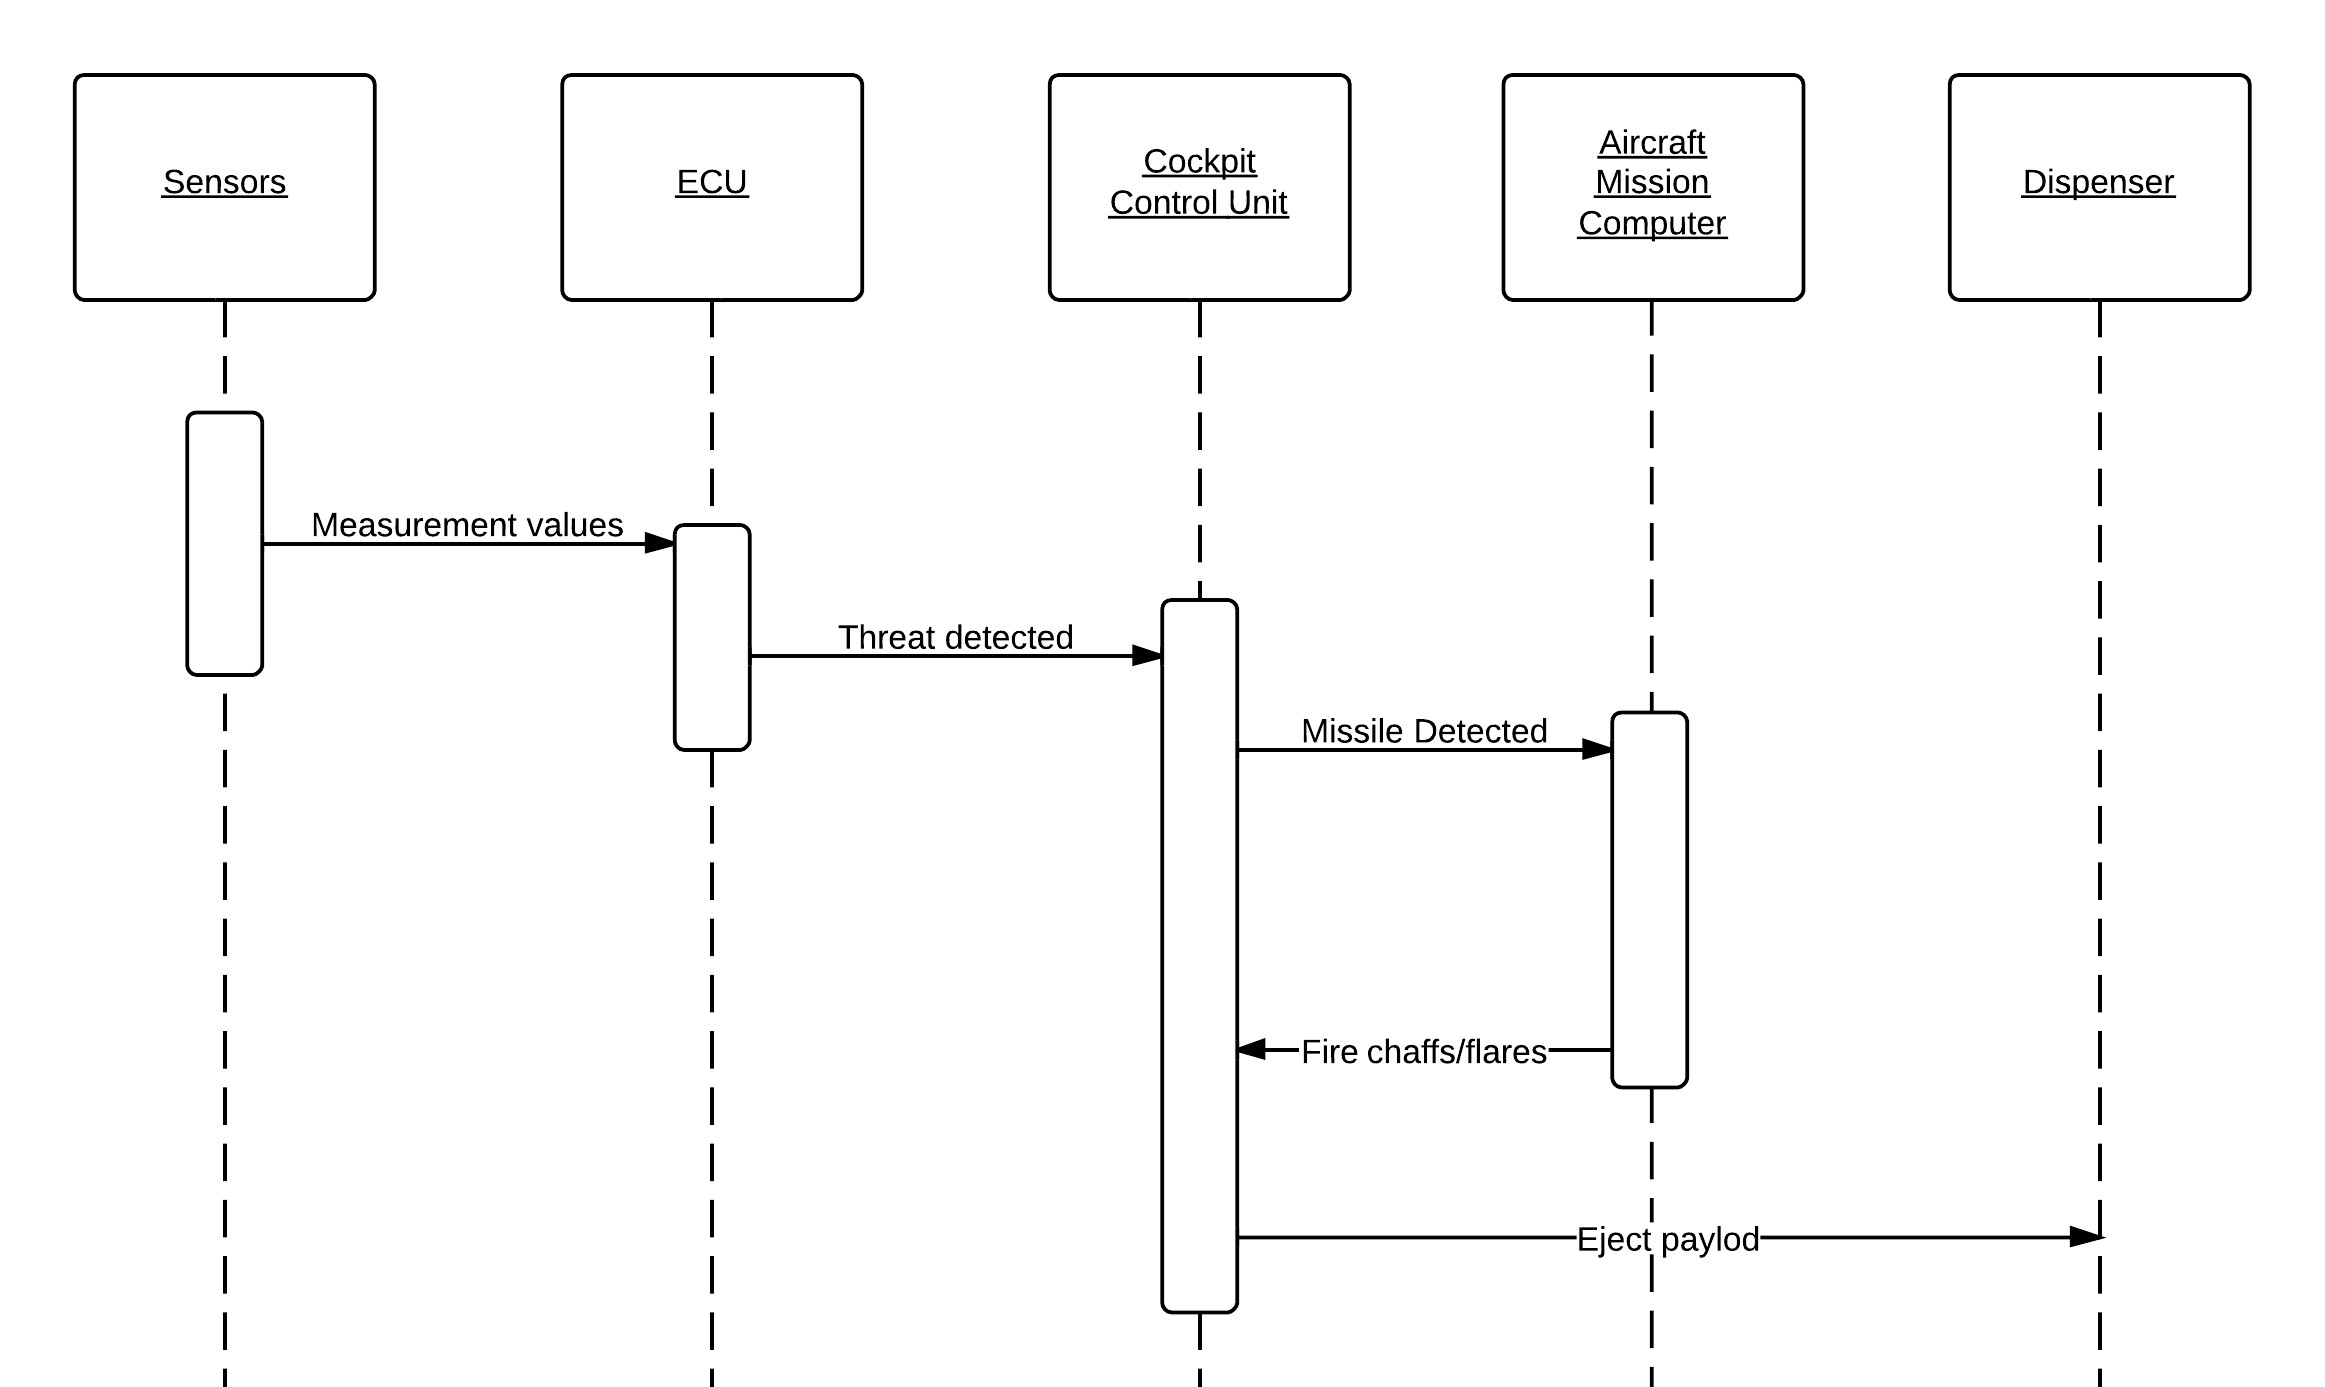
\includegraphics[scale=0.55]{./images/threatDetectedSequenceDiagram.png}\\
%	\caption{Threat detected sequence diagram}
%    \label{fig:threatDetectedSeqDia}
%\end{figure}